\chapter{Columnar Storage for Daily Bars}\label{ch:columnar}

\begin{objectives}
\begin{itemize}
\item describe row and column layouts of \cc{score::db::Bar} down to byte offsets measured on a real compiler;
\item derive how many bytes and cache lines a close-to-close return computation touches in each layout;
\item prove that a sorted, append-only date column answers \cc{scan(start, end)} in $O(\log n+k)$;
\item prove that ISO-8601 date strings sort chronologically, and say what the interface fails to enforce;
\item recognise \cc{IngestionSource} as the Strategy pattern and connect both data paths to it.
\end{itemize}
{\small\color{muted}\textbf{Chapter references:} Copeland and Khoshafian~\cite{copeland1985dsm}; Stonebraker et al.~\cite{stonebraker2005cstore};
Boncz et al.~\cite{boncz2005x100}; Abadi et al.~\cite{abadi2008colrow,abadi2013design}; Gamma et al.~\cite{gamma1994design};
Glasserman~\cite{glasserman2003monte}; Kx~\cite{kxq}.}
\end{objectives}

\section{The workload decides the layout}
Decision D8 named the two consumers: pre-trade risk checks and backtests. Both ask the same question, ``give me the closes
of \emph{one} symbol between two dates'', and then run arithmetic down that sequence (\cref{ch:risk}). Neither ever asks
for ``all fields of one bar''. That asymmetry is the whole case for a column store.

\repo[firstline=8,lastline=16]{include/score/db/bar.hpp}{One daily OHLCV row. The date is a \cc{std::string} holding
\texttt{"YYYY-MM-DD"}.}{lst:bar}

\repo[firstline=10,lastline=30]{include/score/db/column_store.hpp}{The storage contract. It commits to append and
range-scan semantics but deliberately not to a byte layout; \cc{ColumnStoreV1} currently throws from every method.}{lst:colstore}

\begin{definition}[Row store, column store~\cite{copeland1985dsm}]\label[definition]{def:rowcol}
For a relation with attributes $A_1,\dots,A_d$ and tuples $t_1,\dots,t_n$, a \emph{row layout} stores
$t_1[A_1],\dots,t_1[A_d],t_2[A_1],\dots$ contiguously; a \emph{column layout} stores, for each attribute separately,
$t_1[A_j],t_2[A_j],\dots,t_n[A_j]$ contiguously. Copeland and Khoshafian called the fully decomposed form the
Decomposition Storage Model.
\end{definition}

\section{The bytes, measured}
On the measurement machine (Apple clang 21, libc++, arm64) we compiled \cc{Bar} and printed its layout.

\begin{progout}{layout.cpp: sizeof and offsetof for score::db::Bar}{lst:layoutout}
sizeof(std::string)=24 sizeof(Bar)=64 alignof(Bar)=8
offsets: date=0 open=24 high=32 low=40 close=48 volume=56
PackedRow sizeof=48 offsets date=0 open=8 close=32 volume=40
SSO: string data inside object? 1 (capacity 22)
\end{progout}

The 10-character date fits libc++'s short-string buffer (capacity 22), so it lives inside the 24-byte \cc{std::string}
object and \cc{Bar} is exactly one 64-byte cache line. \cc{PackedRow}, a hypothetical on-disk row with the date as
\cc{int32} days, still occupies 48 bytes because the following \cc{double} must be 8-aligned.

\begin{figure}[htbp]
\centering
\begin{tikzpicture}[x=0.17cm,y=0.75cm]
  \node[font=\small\bfseries,text=fg,anchor=west] at (0,1.2) {Row layout: \texttt{std::vector<Bar>}, 64 bytes per bar};
  \foreach \r in {0,1,2}{
    \pgfmathtruncatemacro{\y}{-\r}
    \draw[draw=muted,fill=codebg] (0,\y) rectangle (24,\y+0.75); \node[font=\scriptsize\ttfamily,text=muted] at (12,\y+0.37) {date (24)};
    \foreach \x/\l in {24/open,32/high,40/low}{\draw[draw=muted,fill=codebg] (\x,\y) rectangle ++(8,0.75); \node[font=\scriptsize\ttfamily,text=muted] at (\x+4,\y+0.37) {\l};}
    \draw[draw=red,fill=red!30!bg,thick] (48,\y) rectangle ++(8,0.75); \node[font=\scriptsize\ttfamily,text=fg] at (52,\y+0.37) {close};
    \draw[draw=muted,fill=codebg] (56,\y) rectangle ++(8,0.75); \node[font=\scriptsize\ttfamily,text=muted] at (60,\y+0.37) {vol};
    \node[font=\scriptsize,text=muted,anchor=east] at (-0.5,\y+0.37) {bar \r};
  }
  \node[font=\scriptsize,text=red,anchor=west] at (65,-0.63) {8 useful bytes per 64-byte line};
  \foreach \x in {0,16,32,48,64}{\node[font=\tiny\ttfamily,text=muted] at (\x,-2.35) {\x};}
  % columns
  \node[font=\small\bfseries,text=fg,anchor=west] at (0,-3.4) {Column layout: one array per field};
  \foreach \i in {0,...,7}{\draw[draw=grn,fill=grn!30!bg,thick] (\i*8,-4.6) rectangle ++(8,0.75); \node[font=\scriptsize\ttfamily,text=fg] at (\i*8+4,-4.23) {c\textsubscript{\i}};}
  \node[font=\scriptsize,text=muted,anchor=east] at (-0.5,-4.23) {close};
  \node[font=\scriptsize,text=grn,anchor=west] at (65,-4.23) {8 closes per 64-byte line};
  \foreach \i in {0,...,7}{\draw[draw=muted,fill=codebg] (\i*8,-5.6) rectangle ++(8,0.75); \node[font=\scriptsize\ttfamily,text=muted] at (\i*8+4,-5.23) {o\textsubscript{\i}};}
  \node[font=\scriptsize,text=muted,anchor=east] at (-0.5,-5.23) {open};
  \node[font=\scriptsize,text=muted,anchor=west] at (65,-5.23) {not read by the query};
\end{tikzpicture}
\caption{Byte-level picture of the two layouts, using the offsets of \cref{lst:layoutout} (TikZ). Red: the close fields a
return computation needs, scattered one per cache line. Green: the same values packed eight per line.}
\label{fig:rowcol}
\end{figure}

\begin{proposition}[Bytes touched by a close-to-close scan]\label[proposition]{prop:bytes}
Let a scan read the close of $k$ consecutive bars, let the row width be $w$ bytes with the close field $f$ bytes wide,
and let cache lines be $L$ bytes with $w\ge L$ and $w$ a multiple of $L$. Then the row layout brings at least
$k$ lines, $kL$ bytes, into cache, while the column layout brings $\lceil kf/L\rceil+1$ lines at most. For $w=L=64$,
$f=8$ the ratio approaches $8$.
\end{proposition}
\begin{proof}
In the row layout the $k$ close fields sit at stride $w\ge L$, so no two of them share a line, and each needs its own line.
In the column layout they occupy $kf$ contiguous bytes, which span at most $\lceil kf/L\rceil+1$ lines (the $+1$ accounts
for a misaligned start). The ratio $kL/(\lceil kf/L\rceil+1)\to L^2/(fL)=L/f=8$.
\end{proof}

\begin{verified}
For the mock generator's $n=504$ bars: row layout $504\times64=32{,}256$ bytes in 504 lines; packed on-disk rows
$504\times48=24{,}192$ bytes; close column $504\times8=4{,}032$ bytes in 63 lines (aligned). Ten years of 252 trading
days for 500 symbols multiplies each by 2500.
\end{verified}

Bytes are only the first advantage. A column of closes is a dense \cc{double} array, which a compiler can vectorise and
a codec can compress (dates are an arithmetic progression with weekend gaps; volumes vary slowly in magnitude).
C-Store~\cite{stonebraker2005cstore} and MonetDB/X100~\cite{boncz2005x100} built whole systems on these
observations; Abadi, Madden and Hachem measured why simply storing rows by column inside a row engine does not capture
the benefit~\cite{abadi2008colrow}; and the survey by Abadi et al.\ covers the design space~\cite{abadi2013design}.

\begin{history}
Column orientation is old. Copeland and Khoshafian's Decomposition Storage Model appeared at SIGMOD in
1985~\cite{copeland1985dsm}. In finance, Kx Systems' kdb+ and its q language have long stored tick data column-wise
for exactly the ``one symbol, one time range, one field'' queries a risk engine issues~\cite{kxq}.
\end{history}

\section{Sorted, append-only columns}
\begin{lemma}[ISO-8601 dates sort chronologically]\label[lemma]{lem:iso}
For valid dates written as zero-padded \texttt{YYYY-MM-DD} strings with four-digit years, lexicographic comparison of
the strings agrees with chronological order.
\end{lemma}
\begin{proof}
All such strings have length 10, with \texttt{-} at positions 4 and 7, so lexicographic order compares
the digits position by position. For fixed-width zero-padded decimal numerals, digit-wise lexicographic order is numeric
order. The fields appear in order of significance (year, month, day), so the string order is the lexicographic order
of the triple $(Y,M,D)$, which is chronological order.
\end{proof}

\begin{pitfall}[title={Pitfall: the lemma has hypotheses}]
\texttt{"2024-5-7"} $>$ \texttt{"2024-05-07"} lexicographically, because \texttt{'5'} $>$ \texttt{'0'}. The interface types the
date as \cc{std::string}, so nothing stops such a value. \cc{append} must validate the format, or the store must keep
dates as integers (\cref{ex:intdate}).
\end{pitfall}

\begin{theorem}[Range scan]\label{thm:scan}
Suppose the date column of a symbol holds $n$ dates $d_1<d_2<\dots<d_n$ (strictly increasing). Then the indices of all
bars with $d_i\in[s,e]$ form a contiguous range $[\ell, u)$ found with $2\lceil\log_2(n+1)\rceil$ comparisons, and
\cc{scan(symbol, s, e)} costs $O(\log n + k)$ where $k=u-\ell$ is the number of bars returned.
\end{theorem}
\begin{proof}
Let $\ell=\min\{i: d_i\ge s\}$ (lower bound) and $u=\min\{i: d_i> e\}$ (upper bound), with the convention $n+1$ if no
such index exists. Because the column is sorted, $d_i\in[s,e]\iff \ell\le i<u$: for $i<\ell$, $d_i<s$; for $i\ge u$,
$d_i>e$; between them, $s\le d_\ell\le d_i\le d_{u-1}\le e$. Each bound is a binary search over $n+1$ candidate
positions, needing $\lceil\log_2(n+1)\rceil$ comparisons. Copying the $k$ bars costs $O(k)$ per column read.
\end{proof}

For $n=504$, $\lceil\log_2 505\rceil=9$ comparisons per bound. The strictness hypothesis is what the interface comment
asks of \cc{append}: reject bars ``out of order or overlap[ping] dates already stored''.

\begin{proposition}[Append preserves sortedness]\label[proposition]{prop:append}
If the stored column is strictly increasing, and an appended batch $b_1<\dots<b_m$ satisfies $b_1>d_n$, the result is
strictly increasing. The check costs $O(m)$ and needs only the last stored date.
\end{proposition}
\begin{proof}
The concatenation is increasing within each part and across the seam, since $d_n<b_1$. Checking means one comparison
with $d_n$ and $m-1$ adjacent comparisons within the batch.
\end{proof}

\section{IngestionSource as a Strategy}\label{sec:gbm}
\repo[firstline=9,lastline=25]{include/score/db/ingestion.hpp}{One interface for any producer of bars. The comment names
both Python paths as future implementations.}{lst:ingestion}

\begin{layman}
A kitchen does not care whether the vegetables came from the market this morning or from the freezer; it cares that they
arrive washed, cut, and labelled the same way. \cc{IngestionSource} is the loading dock: live \cc{yfinance} data and
synthetic GBM data unload through the same door, so the store and the risk code never learn which truck brought them.
\end{layman}

In the vocabulary of Gamma et al.~\cite{gamma1994design}, \cc{IngestionSource} is a \emph{Strategy}: a family of
interchangeable algorithms (``where do bars come from?'') behind one interface, chosen by the caller at run time. The
context object is whatever calls \cc{ingest(store, symbol)}; the \cc{ColumnStore} it receives is itself an abstraction,
so the two hierarchies vary independently (\cref{fig:ingest}).

\begin{figure}[htbp]
\centering
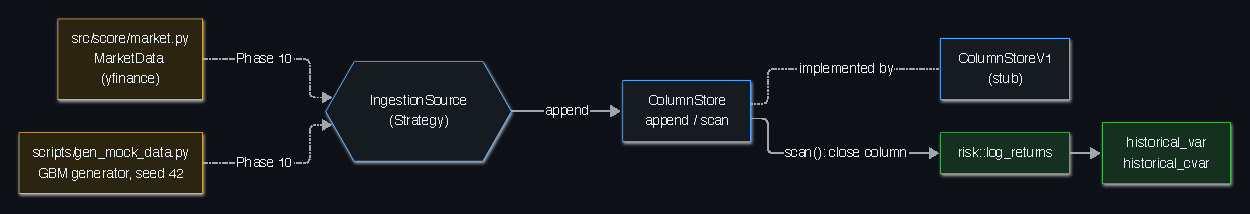
\includegraphics[width=\linewidth]{diagrams/ingestion.pdf}
\caption{Data flow after Phase 10 (Mermaid). Yellow: Python producers, today disconnected. Dotted: bridges that do not
exist yet. Green: the risk code that already works.}
\label{fig:ingest}
\end{figure}

\subsection{The synthetic path, exactly}
\Cref{lst:gbm} implements the solution of the GBM stochastic differential equation $dS=\mu S\,dt+\sigma S\,dW$. By
It\^o's lemma, $\ln S$ is a Brownian motion with drift $\mu-\frac12\sigma^2$ and volatility $\sigma$, so
\[ \ln S_{t+\Delta t}-\ln S_t \sim \mathcal N\!\big((\mu-\tfrac12\sigma^2)\Delta t,\ \sigma^2\Delta t\big) \]
exactly, with independent increments. Simulating in log space therefore has \emph{no discretisation error}, unlike an Euler
step $S_{t+\Delta t}=S_t(1+\mu\Delta t+\sigma\sqrt{\Delta t}Z)$~\cite{glasserman2003monte}. Two details of the code are worth
noticing. First, \cc{np.concatenate(([0.0], np.cumsum(log_increments[:-1])))} uses $N-1$ of the $N$ increments, so the
last normal draw is generated and discarded; the path still has $N$ prices, the first equal to the initial price.
Second, the daily log-returns of the generated closes have model standard deviation $\sigma\sqrt{\Delta t}$, which for
AAPL's $\sigma=0.28$ is $0.28/\sqrt{252}=0.017638$; the realised sample standard deviation of the 503 returns,
computed by the repository's \cc{risk::calculate_risk_from_returns}, is $0.017694$ (\cref{sec:mockvar}).

\begin{exercises}
\ex{ex:ondisk}{\lvC} Design \cc{ColumnStoreV1}'s on-disk layout: one file per (symbol, column), a header with magic,
version, element type and count, then raw little-endian values. Specify the write order (data, \cc{fsync}, header count,
\cc{fsync}) that makes \cc{append} crash-safe, and prove that a crash at any point leaves a store that \cc{scan} reads as
either the old or the new contents.

\ex{ex:bytes500}{\lvA} A nightly batch computes 97.5\% CVaR over 10 years of daily closes for 500 symbols. Compute bytes
read from memory in each layout using \cref{prop:bytes}, and the time at 20\,GB/s of memory bandwidth.

\ex{ex:intdate}{\lvB} Replace the \cc{std::string} date with \cc{int32_t} days since 1970-01-01. Prove that the map from
valid Gregorian dates to day numbers is strictly increasing, give the size of \cc{Bar} after the change (predict, then
check with \cc{sizeof}), and list every place the string form must still exist.

\ex{ex:scanedge}{\lvA} Specify \cc{scan} for: an unknown symbol; $s>e$; $s$ and $e$ both between two stored dates;
malformed date strings. Which should throw \cc{score::DomainError}, and which should return an empty vector? Justify each
from the users named in D8.

\ex{ex:yf}{\lvA} \cc{MarketData} (\cref{lst:market}) fetches \cc{history(period="1d")}. How many log-returns can a
historical VaR compute from that, and what does \cc{historical_var} do with them at $c=0.95$? Specify what a
\cc{YFinanceSource::ingest} must request instead, and how it should avoid re-appending dates already stored.

\ex{ex:compress}{\lvB} Store closes as integer ticks of \$0.0001 (the mock generator rounds to four decimals). Estimate,
from the GBM model, the typical absolute day-to-day change in ticks for AAPL, and hence the bits per value of a
delta-plus-varint encoding (\cref{def:varint}). Compare with 64 bits per \cc{double}.
\end{exercises}

